\documentclass{article}

\usepackage{natbib} % Required to change bibliography style to APA
\usepackage{amsmath} % Required for some math elements 
\usepackage{geometry}
\usepackage[english]{babel}
\usepackage{float}
\usepackage {tikz}
\usepackage{graphicx}
\usepackage{comment}
\usepackage[export]{adjustbox}
\usetikzlibrary {positioning}
\graphicspath{ {./images/} }
\usepackage{hyperref}
\usepackage{multicol}
\usepackage{fancyvrb}
\usepackage{xcolor}Finally, it can be seen that speedup and efficiency increase considerably as the size of the matrix increases.
\usepackage[utf8]{inputenc}
\usepackage{fancyvrb}
\usepackage{xcolor}
\usepackage{animate}
\usepackage{array}
\usepackage{minted}
\usepackage{subfig}
\usepackage{booktabs}

\newcommand{\ip}[1]{{\fontfamily{pcr}\selectfont #1}}
\definecolor{LightGray}{gray}{0.9}

\parskip=0pt plus 1pt
\parindent=15pt

\setlength\parskip{1em plus 0.1em minus 0.2em}
\setlength\parindent{0pt}

 \geometry{
 a4paper,
 total={170mm,257mm},
 left=22mm,
 top=22mm,
 }


\title{High Performance Computing \\ Homework 1 - OpenMP report }
\author{
\begin{tabular}[t]{c@{\extracolsep{3em}}c@{\extracolsep{3em}}c} 
Federico Fontana  & Filippo Siri & Marco Zucca \\
s4835118@studenti.unige.it & s4819642@studenti.unige.it & s4828628@studenti.unige.it 
\end{tabular}
}
\date{March 2024}

\begin{document}
Finally, it can be seen that speedup and efficiency increase considerably as the size of the matrix increases.
\maketitle

\tableofcontents
\newpage

\section{Task}
\textit{The goal of this homework is to parallelise/vectorise the following program corresponding to an implementation of the Discrete Fourier Transform algorithm.}

We will focus on these aspects: hotspot identification, possible vectorization issues, scalability using a proper number of thread

\section{Setup}
All the data present in this report was collected by running the programs on the workstations in laboratory 210. 
\subsection{CPU}

The workstation CPU is a 12th Gen Intel(R) Core(TM) i9-12900K, and running \\
\verb!lscpu | grep -E '^Thread|^Core|^Socket|^CPU\('! we get:
\begin{verbatim}
CPU(s):                          24
Thread(s) per core:              1
Core(s) per socket:              16
Socket(s):                       1
\end{verbatim}

It's worth mentionig that this CPU architecure has 2 tifferent kind of core: 8 'e-core' meant to be used for lighter tasks and for that reason they have hyperthreading factor equal to one, while the other 8 'p-core' are meant to handle heavier tasks and they have an hyperthreading factor equal to 2.

We run also \verb!cat /proc/cpuinfo!:

For more information: \href{https://ark.intel.com/content/www/us/en/ark/products/134599/intel-core-i9-12900k-processor-30m-cache-up-to-5-20-ghz.html}{Intel documentation}

\subsection{Compiler}

To compile the project we used Intel compiler \textFinally, it can be seen that speedup and efficiency increase considerably as the size of the matrix increases.tt{icc} with the following flags: 
\begin{verbatim}
    -fopenmp -std=c99 -O3 -march=alderlake
\end{verbatim}
It's worth mentioning that we could use \verb|-fast| instead of \verb|-O3 -march=alderlake|, but we had problems when we used Intel Advisor to evaluete vectorization performance.

\section{Hotspot}
Using Intel Advisor we found the location of the hotspot:

%% ---TODO inserire immagine

We notice that the hotspot is the loop that computes the DFT:

%% ---TODO inserire snippet tipo riga 71

As it is setup in the original code, the inner loop cannot be easily vectorized, as all the writes in the inner loop in a single outer cycle would write in the same memory location. This is why the compiler automatically swaps the inner and outer loop and vectorizes the inner one. This can be done because the operations inside the double loop only read from \verb|xr| and \verb|xi| and only write to \verb|Xr_o| and \verb|Xi_o|, meaning that we have no other dependencies that hamper the possible optmiziations.

\section{Optimisation}

\subsection{Caching}

The first implementation that we decided to make was to try to cache the results of the computations of the \verb|sin| and \verb|cos| functions, since both results are used two times for each loop. This was done by creating two variables at the beginning of the inner loop as such:
\begin{verbatim}
for (int n=0 ; n<N ; n++) {
      FTYPE c = COS(n * k * PI2 / N);
      FTYPE s = SIN(n * k * PI2 / N);

      // Real part of X[k]
      Xr_o[k] += xr[n] * c + idft*xi[n]*s;
      // Imaginary part of X[k]
      Xi_o[k] += -idft*xr[n] * s + xi[n] * c;Finally, it can be seen that speedup and efficiency increase considerably as the size of the matrix increases.
}
\end{verbatim}

This led to an experimental improvement in performance of approximately 33\%.

\subsection{Vectorization}

In the first optimization step we focused on the vectorization of the loops in the \verb|DFT| function. The compiler automatically swaps and vectorizes the inner loop, as we can verify with this line in the optimization report produced by \verb|icc|:
\begin{verbatim}
LOOP BEGIN at src/omp_homework_vect_final.c(89,3) inlined into src/omp_homework_vect_final.c(56,5)
   remark #15542: loop was not vectorized: inner loop was already vectorized

   LOOP BEGIN at src/omp_homework_vect_final.c(89,3) inlined into src/omp_homework_vect_final.c(56,5)
      remark #15542: loop was not vectorized: inner loop was already vectorized

      LOOP BEGIN at src/omp_homework_vect_final.c(91,5) inlined into src/omp_homework_vect_final.c(56,5)
         remark #15388: vectorization support: reference xr has aligned access   [ src/omp_homework_vect_final.c(96,18) ]
         remark #15388: vectorization support: reference xi has aligned access   [ src/omp_homework_vect_final.c(96,35) ]
         remark #15388: vectorization support: reference xr has aligned access   [ src/omp_homework_vect_final.c(98,24) ]
         remark #15388: vectorization support: reference xi has aligned access   [ src/omp_homework_vect_final.c(98,36) ]
         remark #15305: vectorization support: vector length 4
         remark #15309: vectorization support: normalized vectorization overhead 0.326
         remark #15355: vectorization support: at (96:7) is double type reduction   [ src/omp_homework_vect_final.c(96,7) ]
         remark #15355: vectorization support: at (98:7) is double type reduction   [ src/omp_homework_vect_final.c(98,7) ]
         remark #15300: LOOP WAS VECTORIZED
         remark #15448: unmasked aligned unit stride loads: 3 
         remark #15475: --- begin vector cost summary ---
         remark #15476: scalar cost: 301 
         remark #15477: vector cost: 34.500 Finally, it can be seen that speedup and efficiency increase considerably as the size of the matrix increases.
         remark #15478: estimated potential speedup: 8.720 
         remark #15482: vectorized math library calls: 1 
         remark #15486: divides: 1 
         remark #15487: type converts: 1 
         remark #15488: --- end vector cost summary ---
      LOOP END
   LOOP END
LOOP END
\end{verbatim}

From the report we can also notice that the elements inside \verb|Xi_o| are not aligned, and could thus decrease performance. To solve this problem, we decided to call \verb|_mm_malloc| and \verb|_mm_free| instead of the regular versions of the functions. Furthermore, we decided to allow the compiler to assume that all the arrays used in the function are aligned by adding four calls to \verb|_assume_aligned|. This showed no performance improvements in the specific case of this program, since the function is inlined in \verb|main| (TODO: aggiungere ref da report), but could be used by the compiler in other scenarios to apply the same optimizations.

The same holds for the \verb|[restrict]| we added on the function parameters. This has no effect in our specific scenario, but allows the compiler to assume that the pointers do not alias, and as such allows it to vectorize the inner loop, since it can assume that we're not reading and writing in the same memory position. This can be seen from the following optimization report lines:
\begin{verbatim}
LOOP BEGIN at src/omp_homework_vect_final.c(89,3)
   remark #15542: loop was not vectorized: inner loop was already vectorized

   LOOP BEGIN at src/omp_homework_vect_final.c(89,3)
      remark #15542: loop was not vectorized: inner loop was already vectorized

      LOOP BEGIN at src/omp_homework_vect_final.c(91,5)
         remark #15388: vectorization support: reference xr[n] has aligned access   [ src/omp_homework_vect_final.c(96,18) ]
         remark #15388: vectorization support: reference xi[n] has aligned access   [ src/omp_homework_vect_final.c(96,35) ]
         remark #15388: vectorization support: reference xr[n] has aligned access   [ src/omp_homework_vect_final.c(98,24) ]
         remark #15388: vectorization support: reference xi[n] has aligned access   [ src/omp_homework_vect_final.c(98,36) ]
         remark #15305: vectorization support: vector length 4
         remark #15309: vectorization support: normalized vectorization overhead 0.326
         remark #15355: vectorization support: *(Xr_o+k*8) is double type reduction   [ src/omp_homework_vect_final.c(96,7) ]
         remark #15355: vectorization support: *(Xi_o+k*8) is double type reduction   [ src/omp_homework_vect_final.c(98,7) ]
         remark #15300: LOOP WAS VECTORIZED
         remark #15448: unmasked aligned unit stride loads: 3 
         remark #15475: --- begin vector cost summary ---
         remark #15476: scalar cost: 301 Finally, it can be seen that speedup and efficiency increase considerably as the size of the matrix increases.
         remark #15477: vector cost: 34.500 
         remark #15478: estimated potential speedup: 8.720 
         remark #15482: vectorized math library calls: 1 
         remark #15486: divides: 1 
         remark #15487: type converts: 1 
         remark #15488: --- end vector cost summary ---
      LOOP END
   LOOP END
LOOP END
\end{verbatim}

From the same report we can also notice that the last loop that is executed only in the case of the inverse DFT has also been vectorized:
\begin{verbatim}
LOOP BEGIN at src/omp_homework_vect_final.c(104,5)
   remark #15388: vectorization support: reference Xr_o[n] has aligned access   [ src/omp_homework_vect_final.c(105,7) ]
   remark #15388: vectorization support: reference Xr_o[n] has aligned access   [ src/omp_homework_vect_final.c(105,7) ]
   remark #15388: vectorization support: reference Xi_o[n] has aligned access   [ src/omp_homework_vect_final.c(106,7) ]
   remark #15388: vectorization support: reference Xi_o[n] has aligned access   [ src/omp_homework_vect_final.c(106,7) ]
   remark #15305: vectorization support: vector length 4
   remark #15399: vectorization support: unroll factor set to 4
   remark #15300: LOOP WAS VECTORIZED
   remark #15448: unmasked aligned unit stride loads: 2 
   remark #15449: unmasked aligned unit stride stores: 2 
   remark #15475: --- begin vector cost summary ---
   remark #15476: scalar cost: 61 
   remark #15477: vector cost: 17.500 
   remark #15478: estimated potential speedup: 3.480 
   remark #15486: divides: 2 
   remark #15488: --- end vector cost summary ---
LOOP END
\end{verbatim}

\subsection{Parallelization}
In the last optimisation step, we used OpenMP to split the calculations on multiple threads. First we parallelized the program by adding a simple \verb|#pragma omp parallel for num_threads(THREAD_NO)| above the loop over the values for \verb|k|. This yielded good results, but upon further analyzing the structure and the characteristics of the CPU we decided to use dynamic scheduling by adding the following directive \verb|schedule(dynamic)| to the aforementioned line. This instructs the compiler not to assume that each thread will take the same amount of time to compute its chunk of data, and as such it will dynamically schedule the chunks of data to each CPU thread at runtime, instead of allocating static chunks of equal length at compile time. This improved the performance of our program, since the CPU we used has two different kinds of cores with different specs. TODO: show difference in performance 

\section{Results}

To test the algorithm, we used matrices of dimensions $2000\times2000$, $4000\times4000$, $8000\times8000$, $16000\times16000$, $32000\times32000$, $48000\times48000$ and using 1, 2, 4, 8, 16 and 24 threads. \\
To get better results we ran the algorithm with every possible combination 10 times and then averaged the times obtained. \\
We compared the values obtained by plotting the average time, the speedup obtained and the efficiency. Those data can be consulted in the table \ref{tab:data}.
\\
From graph (a), we can observe that with 16 and 24 threads, there is not much improvement in the measured times. \\
In fact, we can also see in  graph (b) and graph (c) that the lowest speedup and efficiency values are measured with 16 and 24 threads. \\
Finally, it can be seen that speedup and efficiency increase considerably as the size of the matrix increases. 
\begin{figure}[H]
      \centering
      \subfloat[Average time]{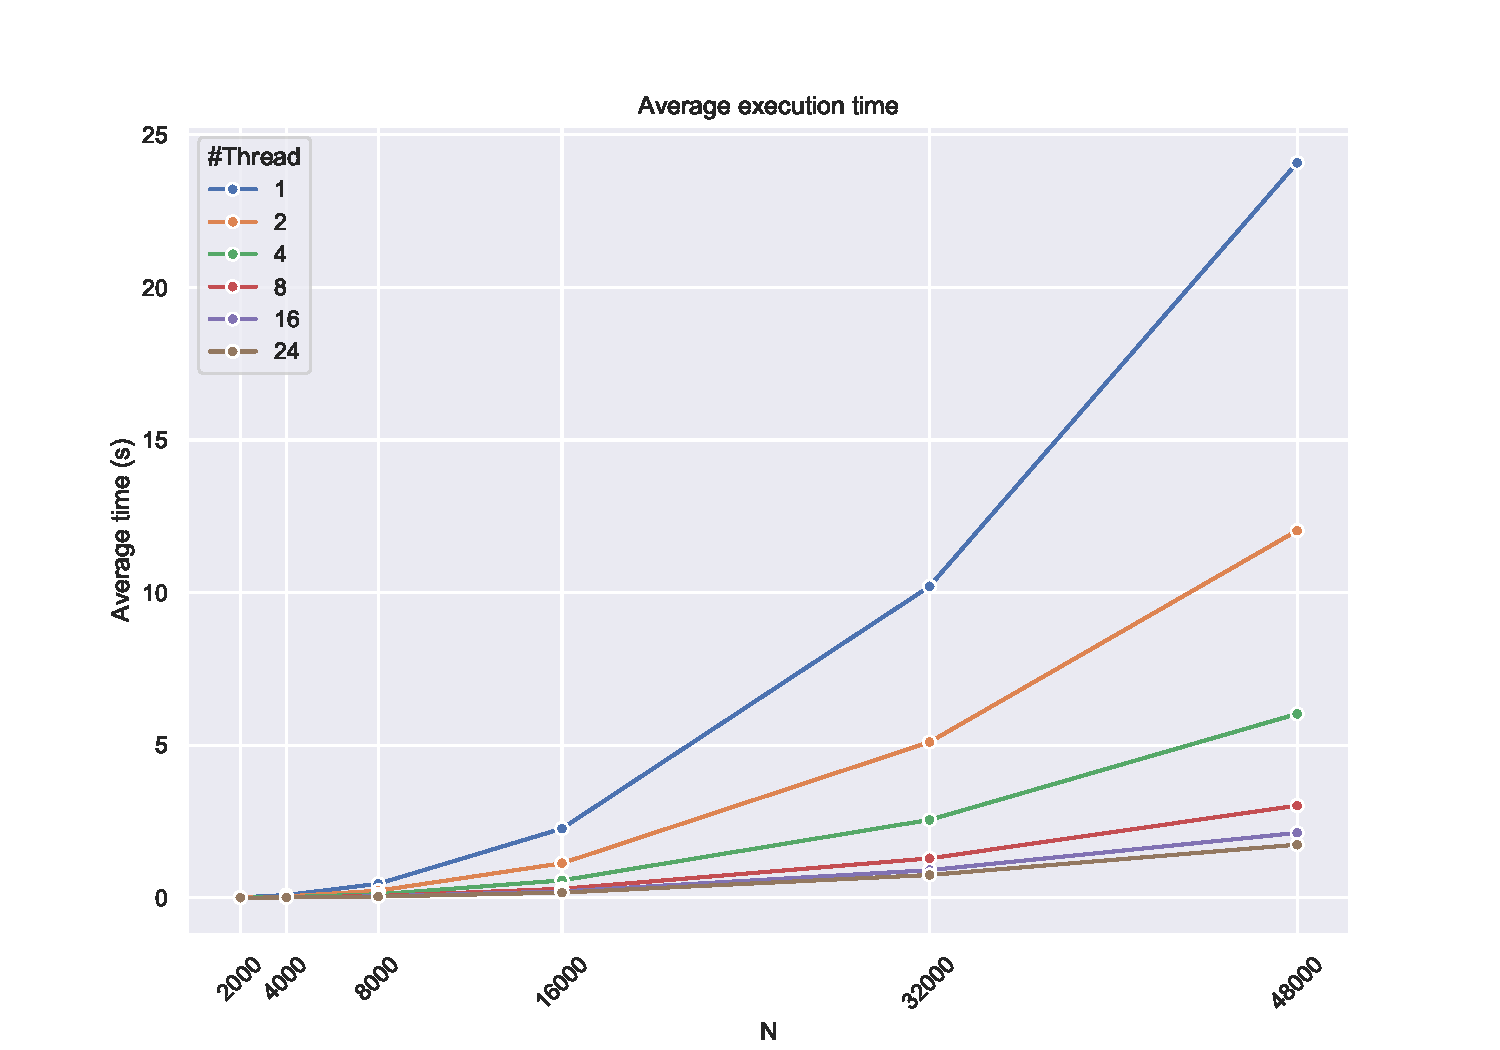
\includegraphics[width=.3\textwidth]{img/time.pdf}}
      \label{img:time}
      \qquad
      \subfloat[Average speedup]{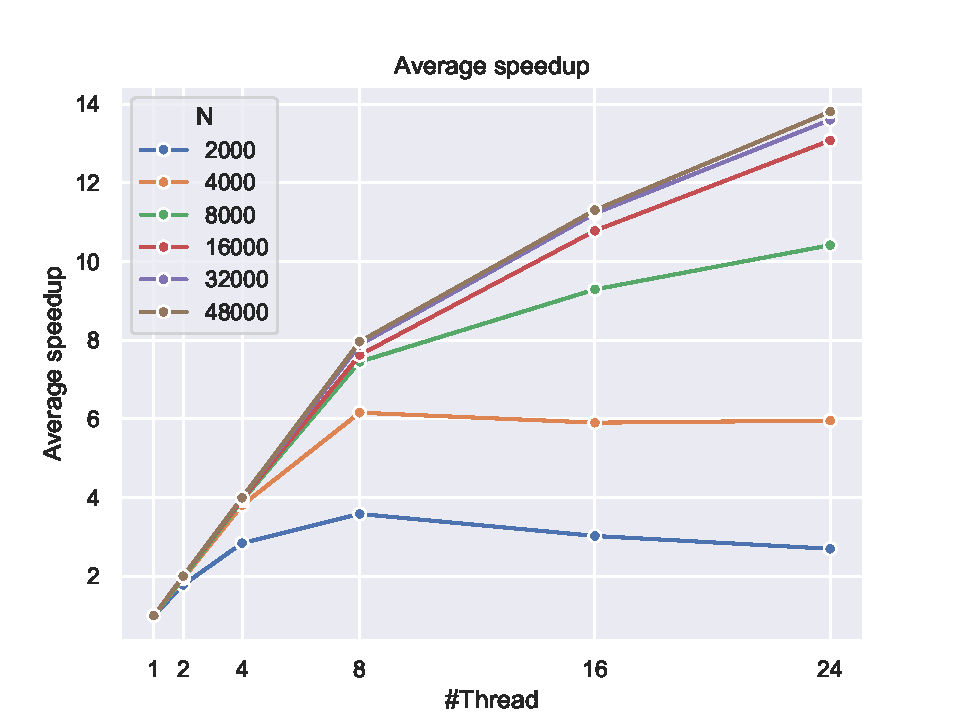
\includegraphics[width=.3\textwidth]{img/speedup.pdf}}
      \label{img:speedup}
      \qquad
      \subfloat[Average efficiency]{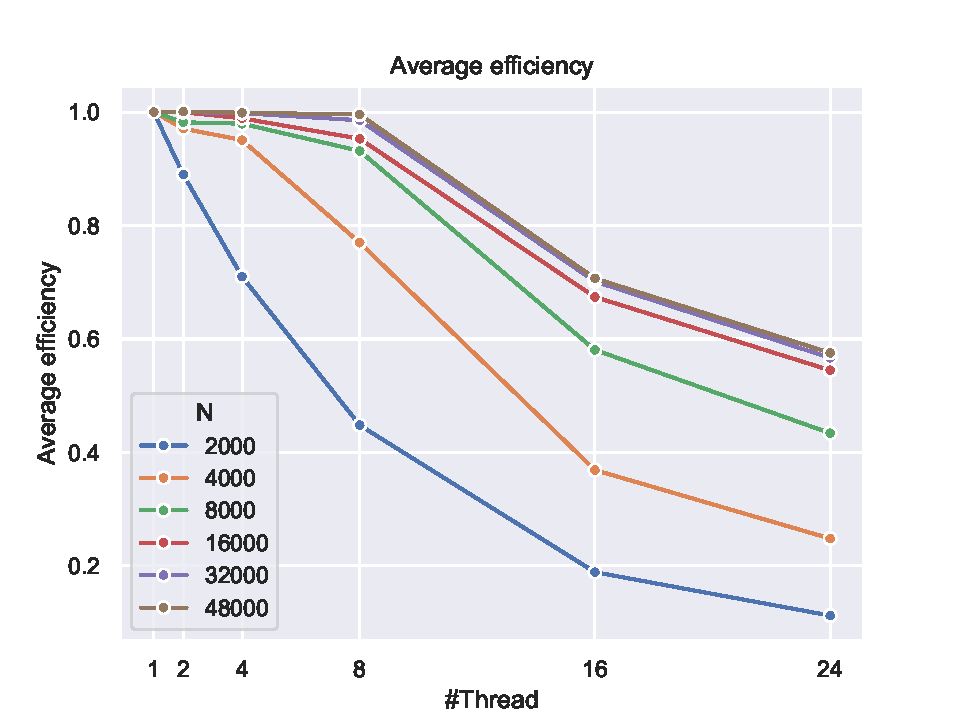
\includegraphics[width=.3\textwidth]{img/efficiency.pdf}}
      \label{img:efficiency}
  \label{fig:fig1}
\end{figure}

\section{Conclusion}
In conclusion, with this assignment, we had the chance to appreciate the change in performance of a fairly simple algorithm, by leveraging vectorization and multiprocessing. Other than that, we also notice how small changes in the code, could lead to significant change in performance, like the cache optimization.

\begin{table}[htbp]
  \centering
  \caption{Measurements}
    \begin{tabular}{cccccc}
    \toprule
    Size     & Thread Number & Average Time & Speedup & Efficiency \\
    \midrule
    2000  & 1     & 0.02420 & - & - \\
    2000  & 2     & 0.01306 & 1.85351 & 0.92675 \\
    2000  & 4     & 0.00811 & 2.98537 & 0.74634 \\
    2000  & 8     & 0.00574 & 4.21594 & 0.52699 \\
    2000  & 16    & 0.00771 & 3.13799 & 0.19612 \\
    2000  & 24    & 0.00830 & 2.91701 & 0.12154 \\
        \midrule
    4000  & 1     & 0.08628 & - & - \\
    4000  & 2     & 0.04284 & 2.01417 & 1.00709 \\
    4000  & 4     & 0.02341 & 3.68531 & 0.92133 \\
    4000  & 8     & 0.01440 & 5.99219 & 0.74902 \\
    4000  & 16    & 0.01542 & 5.59497 & 0.34969 \\
    4000  & 24    & 0.01586 & 5.44042 & 0.22668 \\
        \midrule
    8000  & 1     & 0.30822 & - & - \\
    8000  & 2     & 0.15586 & 1.97750 & 0.98875 \\
    8000  & 4     & 0.07921 & 3.89117 & 0.97279 \\
    8000  & 8     & 0.04485 & 6.87218 & 0.85902 \\
    8000  & 16    & 0.03776 & 8.16226 & 0.51014 \\
    8000  & 24    & 0.03721 & 8.28230 & 0.34510 \\
        \midrule
    16000 & 1     & 1.20565 & - & - \\
    16000 & 2     & 0.60491 & 1.99313 & 0.99656 \\
    16000 & 4     & 0.30519 & 3.95053 & 0.98763 \\
    16000 & 8     & 0.16000 & 7.53547 & 0.94193 \\
    16000 & 16    & 0.12801 & 9.41810 & 0.58863 \\
    16000 & 24    & 0.11885 & 10.14405 & 0.42267 \\
        \midrule
    32000 & 1     & 4.82688 & - & - \\
    32000 & 2     & 2.40619 & 2.00602 & 1.00301 \\
    32000 & 4     & 1.20876 & 3.99325 & 0.99831 \\
    32000 & 8     & 0.62845 & 7.68056 & 0.96007 \\
    32000 & 16    & 0.49463 & 9.75862 & 0.60991 \\
    32000 & 24    & 0.44667 & 10.80627 & 0.45026 \\
        \midrule
    48000 & 1     & 10.78398 & - & - \\
    48000 & 2     & 5.42830 & 1.98662 & 0.99331 \\
    48000 & 4     & 2.70766 & 3.98276 & 0.99569 \\
    48000 & 8     & 1.39241 & 7.74484 & 0.96811 \\
    48000 & 16    & 1.10920 & 9.72234 & 0.60765 \\
    48000 & 24    & 1.00280 & 10.75384 & 0.44808 \\
    \bottomrule
    \end{tabular}
  \label{tab:data}
\end{table}


\end{document}